\section{The algorithmic agent}


\begin{frame}[label=ladila]{The algorithmic agent}
 \begin{center}
  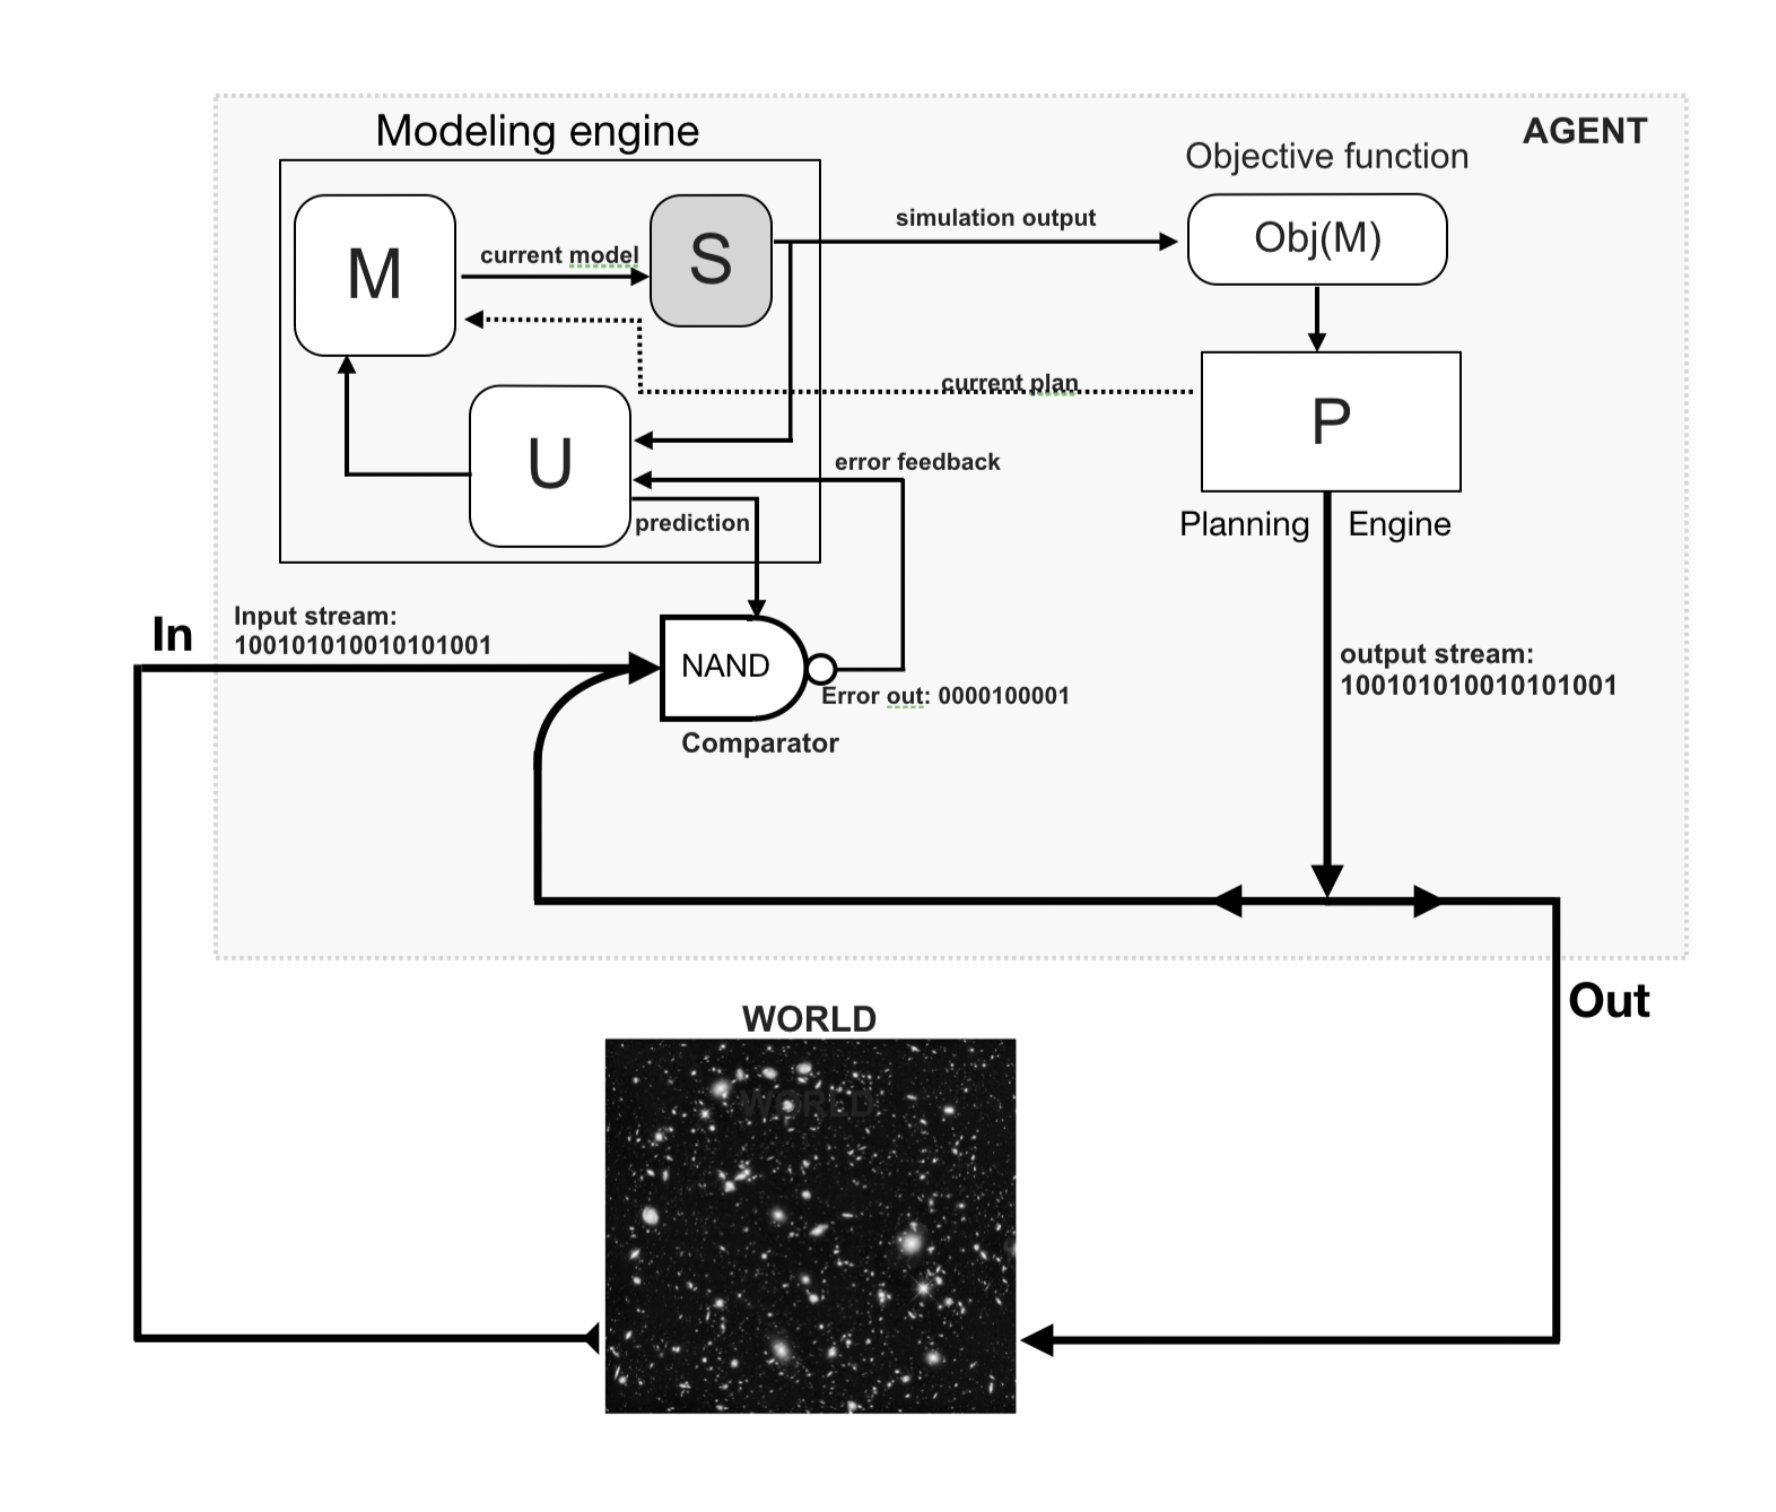
\includegraphics[height=8cm]{img/agent.png}
  \end{center}
  
 %The Modeling engine runs the Model and makes predictions of future data, and then evaluates the prediction error (from the Comparator) to update the Model.  The modeling engine includes three blocks. One holds the current Model state (M), which is used by the simulation engine (S). The simulation engine is used to run simulations of future inputs and outputs to estimate the state of the objective function. It is also used by the Planning engine to run counterfactual simulations and select a Plan and the next actions (outputs). The Update module (U) receives as inputs prediction errors from the Comparator and updates the Model. 
 
 %The other agent elements are the Objective Function, which the agent aims to optimize through a choice of actions as specified by the Planning Engine (P), which develops action strategies and creates efferent signals (outputs). The agent interacts dynamically with its environment, and is involved in a continuous exchange of data with the external world
\end{frame}


\begin{frame}[label=ladila]{Model-building: life}
 How do agents build models? In addressing this question, the algorithmic framework connects the concepts of life, intelligence, and \SEP. Both life and intelligence represent processes to construct simple models for the perdurance of algorithmic information-preserving systems across time. \vfill
 
  Starting from resilient building blocks, from a computational perspective {\em life} is an algorithmic process: program building carried not solely by the individual agent, but by the trans-generational agent through evolution (v. also \cite{Walker2013, Chaitin2012-wd}).
  
\end{frame}

\begin{frame}[label=ladila]{Model-building: intelligence}
 Evolutive pressure gives rise to the next leap, {\em intelligence}: agents that, starting from their static model (DNA in life) can actually build higher-level compressive models of the world within their lifetime, e.g., using brains.\vfill
 
 Importantly, KT holds that both static-model and active-modeling agents enjoy structured experience, only that their level of structure is different. 
\end{frame}


\begin{frame}[label=ladila]{Model-building in artificial agents}
As a consequence of the above, two routes to the construction of model-building agents   (virtual or physical)  should be investigated: \vfill

A) {\bf Single generation} model building where agents are endowed with simplicity biases for model building (this is what we call the  {\em intelligence} approach). \vfill


B) {\bf Trans-generational} model building ({\em life}) where the bias for simplicity is not added by hand but emerges naturally from the construction process that favors simple short programs (and which then lead to phenotype symmetry as in \citep{Johnston2022})  and evolutionary pressure in {\em  environments governed by simple laws}.  
\end{frame}